\section{Частично наблюдаемые среды}\label{sec:PoMDP}

\subsection{Частично наблюдаемые MDP}

Рассматривавшиеся MDP до этого являлись \emph{полностью наблюдаемыми} (fully observable): агенту в качестве наблюдения было доступно всё состояние целиком. Конечно, это довольно-таки существенное упрощение.

\begin{definition}
MDP называется \emph{частично наблюдаемым} (partially observable, принятое сокращение --- PoMDP), если дополнительно задано множество $\mathcal{O}$, называемое \emph{пространством наблюдений} (observation space), и распределение $p(o \mid s)$, определяющая вероятность получить то или иное наблюдение агента $o \in \mathcal{O}$ в момент времени, когда мир находится в состоянии $s \in \St$.
\end{definition}

Если MDP --- <<управляемая>> марковская цепь, то PoMDP можно рассматривать как <<управляемую>> \href{https://en.wikipedia.org/wiki/Hidden_Markov_model}{скрытую марковскую цепь}: действия влияют на то, как будут порождаться следующие состояния, но для наблюдения доступны не сами состояния, а только какие-то другие случайные величины, про которые, однако, известно, что они зависят только от текущего состояния. При этом состояния всё также удовлетворяют свойству марковости, а функция переходов и процесс генерации наблюдений по состоянию --- свойству стационарности.

В PoMDP стратегия должна уметь принимать решение на основании не только текущего наблюдения, но всей истории цепочки наблюдений, так как в них может содержаться информация о текущем состоянии среды. Естественно, эта задача более приближена к реальности, но сильно сложнее. Агенту теперь нужна <<модель памяти>>, способ хранения и учёта всей истории в течение эпизода.

Заметим, что награда по своему определению наблюдаема. Если раньше можно было считать, что награда --- часть состояния, то теперь награда <<по логике>> модели есть часть наблюдений, а значит, формально может рассматриваться как функция от наблюдений. Далее будем работать в соглашении, что награда --- детерминированная функция от наблюдений.

\subsection{Belief MDP}

Допустим, задано PoMDP, и нам доступны все распределения (вероятности переходов и вероятности наблюдений). Пусть мы знаем вероятность $p(s_0)$, какое состояние генерируется изначально (будем считать, стохастично). Допустим, начался новый эпизод, и мы получили наблюдение $o_0 \in \mathcal{O}$. Что мы можем сказать о том, в каком состоянии $s_0$ мы на самом деле оказались? Ответ на этот вопрос формально даёт формула Байеса:
\begin{equation}\label{initial_belief}
p(s_0 \mid o_0) = \frac{p(o_0 \mid s_0)p(s_0)}{\int_{\mathcal{O}} p(o_0 \mid s_0)p(s_0) \diff o_0}
\end{equation}
Здесь в числителе стоит вероятность первого наблюдения и априорное распределение на состояниях, а в знаменателе стоит нормировочная константа. Пока будем считать, что мы умеем брать любые интегралы (например, если пространства состояний и наблюдений конечны и малы).

Допустим, мы выбрали действие $a_0$, попали в состояние $s_1$ (которое мы не видим) и получили наблюдение $o_1$. Что мы можем сказать о том, в каком состоянии $s_1$ мы находимся? Опять же, пользуясь формулой Байеса и используя вероятностную модель PoMDP, мы можем получить точную формулу наших представлений о том, в каком состоянии на текущий момент пребывает агент. Чтобы проделать вывод, обозначим за $\Traj_{:t}$ наблюдаемую (действия, награды, наблюдения, но не состояния) траекторию до момента времени $t$, включая последнее наблюдение:
$$\Traj_{:t} \coloneqq (o_0, a_0, r_0, o_1, a_1, r_1 \dots o_{t - 1}, a_{t - 1}, r_{t - 1}, o_t)$$

\begin{definition}
Вероятность пребывания в том или ином состоянии при условии наблюдаемой истории $p(s_t \HM\mid \Traj_{:t})$ называется \emph{belief state} и сокращённо обозначается $b_t$.
\end{definition}

По определению $b_0(s_0) \HM= p(s_0 \HM\mid o_0)$, которую мы получили в по формуле Байеса в \eqref{initial_belief}. Как обновить belief state после совершения одного шага в среде (получения одного наблюдения и выбора одного действия)?

\begin{theorem}
С точностью до нормировочной константы:
\begin{equation}\label{beliefupdate}
b_t(s_t) \propto p(o_{t} \mid s_{t})\int\limits_{\St} p(s_t \mid s_{t - 1}, a_{t - 1})b(s_{t - 1}) \diff s_{t - 1}
\end{equation}
\begin{proof}
Нашей целью является посчитать $b_t(s_t) \HM\coloneqq p(s_t \HM\mid \Traj_{:t}) \HM= p(s_t \HM\mid o_t, a_{t-1}, \Traj_{:{t-1}})$. Применим формулу Байеса:
$$b_t(s_t) \propto p(o_t \mid s_t, a_{t-1}, \Traj_{:{t-1}})p(s_t \mid a_{t-1}, \Traj_{:{t-1}}) = (*)$$

Первый множитель здесь по определению вероятностной модели есть $p(o_t \mid s_t)$, а во втором множителе, чтобы воспользоваться функцией переходов, нужно проинтегрировать по неизвестному нам предыдущему состоянию $s_{t - 1}$:
\begin{align*}
(*) 
&= p(o_t \mid s_t) \int\limits_{\St} p(s_t, s_{t - 1} \mid a_{t - 1}, \Traj_{:{t-1}}) \diff s_{t - 1} = \\ 
&= p(o_t \mid s_t) \int\limits_{\St} p(s_t \mid s_{t - 1}, a_{t - 1})p(s_{t - 1} \mid \Traj_{:{t-1}}) \diff s_{t - 1}
\end{align*}

Осталось заметить, что по определению $p(s_{t - 1} \mid \Traj_{:{t-1}}) = b_{t - 1}(s_{t - 1})$ --- информация о текущем состоянии с прошлого шага.
\end{proof}
\end{theorem}

\begin{exampleBox}[righthand ratio=0.6, sidebyside, sidebyside align=center, lower separated=false]{}
Допустим, в PoMDP с 10 состояниями и действиями вправо-влево получаем детерминировано в качестве наблюдения бинарный флаг: есть ли пальма или нет. Начальное состояние определяется случайно равномерно. Посмотрим, как меняется belief state, если агент заспавнился в самом левом состоянии и дальше выбирает действия <<вправо>>.

\tcblower
\animategraphics[controls, width=\linewidth]{1}{Images/BeliefMDP/BeliefMDP-}{1}{5}
\end{exampleBox}

Belief state --- <<достаточная статистика>> для описания всей предыдущей истории. Посчитав его, мы собрали абсолютно всю имеющуюся у нас информацию. Это замечание позволяет формально свести задачу в PoMDP к обычному MDP, но требует знания всех распределения и возможности пересчитывать belief state:

\begin{definition}
Для данного PoMDP \emph{Belief MDP} называется следующее MDP:
\begin{itemize}
    \item Пространством состояний является пространство $\Prob(\St)$ распределений в $\St$;
    \item Пространством действий является $\A$;
    \item Функция переходов $p(b' \mid b, a)$, где $b, b' \in \Prob(\St)$ устроена так: сэмплируются $s \HM\sim b(s)$, $s' \HM\sim p(s' \HM\mid s, a)$, $o' \HM\sim p(o' \mid s')$, после чего новый belief state рассчитывается по формуле:
    $$b'(s') \propto p(o' \mid s')\int\limits_{\St} p(s' \mid s, a) b(s) \diff s $$
    \item Функция награды для текущего состояния $b$ и действия $a$ устроена так: для того же сэмпла $s$, использованного в переходе, выдаётся награда $r(s, a)$.
\end{itemize}
\end{definition}

Теория Belief MDP позволяет предложить алгоритмы динамического программирования наподобие Value Iteration и Policy Iteration для решения задач в PoMDP. Однако, в реальности работать с Belief MDP в средах со сложным пространством состояний довольно неудобно: если все распределения неизвестны, интегралы в формуле обновления \eqref{beliefupdate} не берутся, и даже просто хранить <<распределение над состояниями>> невозможно, то не совсем понятно, что можно извлечь от этой теории в сложных средах. Понятно, что при взаимодействии со средой агент должен помимо прочего стремиться выполнять те действия, которые дают наибольшую информацию о belief state, и позволяют <<локализоваться>> в пространстве состояний.

\subsection{Рекуррентные сети в Policy Gradient}

Видимо, поэтому пока самое распространённое решение для работы в PoMDP --- добавление в архитектуры моделей рекуррентных слоёв (GRU или LSTM). При использовании рекуррентных стратегий скрытое состояние инициализируется нулевым вектором в начале каждого эпизода и <<хранит всю необходимую информацию>> о предыдущих наблюдениях, а все модели на вход получают лишь то, что поступает с сенсоров. Де-факто все наши модели оценочных функций и стратегии становятся функциями от всей истории $o_0, o_1, o_2 \dots o_t$. Обсудим, как это меняет ранее встречавшиеся алгоритмы.

Чистые on-policy алгоритмы, такие как REINFORCE, A2C и мета-эвристики, практически не меняются. В A2C лишь стоит иметь в виду, что градиенты текут только по тому роллауту, который собран на текущей итерации; таким образом, агенту будет тяжело научиться запоминать информацию дольше, чем на $N$ шагов, где $N$ --- длина роллаутов.

В PPO скрытое состояние модели сохраняется для всего собранного датасета. Далее из датасета сэмплируются не мини-батчи, а мини-батчи роллаутов (некоторой длины $N$). Затем скрытое состояние инициализируется сохранённым значением при сборе датасета (поскольку стратегия <<не меняется сильно>>, считается, что это сохранённое состояние более-менее не устарело), и модель прогоняется на засэмплированном роллауте для подсчёта всех градиентов.

\subsection{R2D2}

В off-policy алгоритмах сохранять значение скрытого состояния в реплей буфере на первый взгляд бессмысленно; модель может изменится сколько угодно сильно, и сохранённые значения памяти будут неактуальны. С течением обучения скрытое состояние рекуррентных сетей просто меняет своё семантическое значение: модель со свежими весами просто по-другому будет интерпретировать латентное представление.

Рассмотрим две эвристики для преодоления этой проблемы из алгоритма R2D2. Из реплей буфера генерируются роллауты некоторой длины $N$. Скрытое состояние инициализируется сохранённым в буфере значением (которое потенциально <<протухло>>). Модель прогоняется заново на всём роллауте, но функция потерь и backpropagation считается лишь на последних $M \HM< N$ шагов. Таким образом обучение проводится стандартным для рекуррентных сетей подходом backpropagation through time (BPTT).

Первые же $N \HM- M$ шагов нужны исключительно для <<\emph{прогрева}>> (burn-in) скрытого состояния, чтобы его семантическое значение начало более-менее соответствовать свежим весам модели. Это не так дорого вычислительно, как заново прогонять модель по всему эпизоду; так можно было бы получить <<честные>> актуальные значения памяти, но параллелизовать такие вычисления по батчу, в котором встречаются роллауты из разных моментов эпизодов, неудобно и достаточно дорого. Естественно, аналогичный прогон проводится для таргет-сети.

\begin{center}
    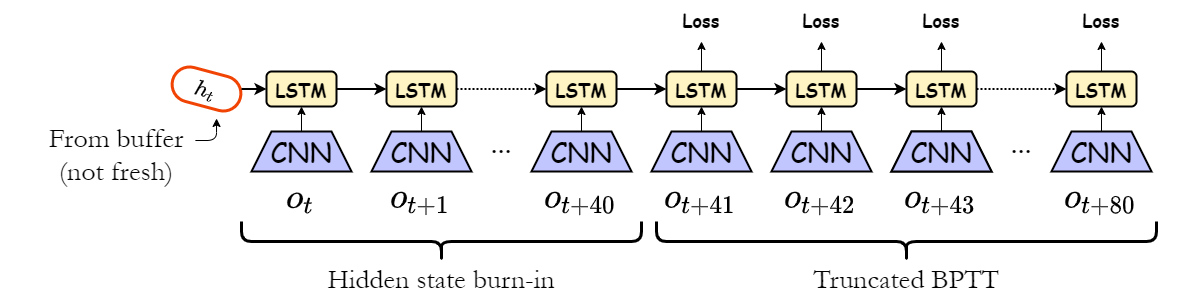
\includegraphics[width=0.9\textwidth]{Images/R2D2.png}
\end{center}

Вторая эвристика заключается в том, чтобы <<разогретое>> состояние после $N \HM- M$ шагов сохранить в буфере для того роллаута, который начинается с соответствующего перехода, и таким образом сделать сохранённое значение чуть более актуальным.

Как обычно, длина $M$ той части траектории, вдоль которой пропускаются градиенты, и ограничивает то время, <<на которое>> агент может теоретически научиться что-то запоминать. Однако, увеличивать его может быть чревато не только тем, что алгоритм станет вычислительно сложным, но и тем, что в батче оказываются $M$ очень похожих друг на друга переходов, и перебивать эту скоррелированность лоссов придётся размером мини-батча.

\begin{remark}
Может быть удобно для ускорения сэмплирования хранить в реплей буфере эпизоды, уже разбитые на фрагменты удобного размера. Например, авторы R2D2 выбирают $N \HM= 80$, $M \HM= 40$, и при сборе данных собирают 40 последовательных переходов, которые упаковываются в буфер единым комплектом; из-за такой оптимизации промежуточные переходы в этом роллауте никогда не будут засэмплированы для обучения как, например, стартовые (с которых начинается роллаут из $N$ шагов). Кажется, что что немного нарушает <<симметричность>> данных, но похоже, что это не так критично, зато сильно упрощает код и сэмплирование мини-батчей.
\end{remark}

\subsection{Neural Episodic Control (NEC)}

\emph{Эпизодичная память} означает, что вместо (или дополнительно к) рекуррентных связей в качестве памяти используется набор ранее встретившихся состояний или их латентных описаний. Механизм работы с такой памятью очень схож с механизмом внимания. Рассмотрим алгоритм Neural Episodic Control в качестве примера применения такой идеи.

Для каждого действия $a$ будем хранить словарь, то есть некоторый набор ключ-значение $M_a \coloneqq (k, v)$. Ключом $k \in \R^d$ является вектор-эмбеддинг, описывающий некоторое состояние $s$ из опыта агента. Значением $v$ является скаляр, оценивающий $Q^*(s, a)$.

При взаимодействии со средой агент действует следующим образом. Текущее состояние $s$ подаётся на вход сети с параметрами $\theta$, которая выдаёт его описание $q(s, \theta) \in \R^d$. Выходом $Q^*(s, a)$ модели является результат применения \emph{механизма внимания} (attention) к словарю $M_a$ с запросом $q(s, \theta)$: для каждого ключа $k$ в словаре определяется похожесть запроса на ключ $\rho(q(s, \theta), k)$ при помощи некоторой функции близости $\rho$, например:
$$\rho(q, k) \coloneqq \frac{1}{\|q - k\|_2^2 + \delta},$$
где $\delta$ --- небольшая константа для защиты от деления на ноль. Затем для каждой пары ключ-значение определяется его вес:
$$w(k) \propto \rho(q, k),$$
где нормировочная константа вычисляется из соображения $\sum_{k, v \in M_a} w(k) = 1$. Наконец, выход дифференцируемого чтения из словаря определяется как сумма значений с вычисленными весами:
$$Q^*(s, a, \theta) \coloneqq \sum_{k, v \in M_a} w(k)v$$

Поскольку размер словаря может быть достаточно большой, а процедуру нужно проводить для каждого $a \in \A$, предлагается использовать в формуле две аппроксимации. Во-первых, учитываются только топ-50 самых значимых (имеющих наибольший вес $w(k)$) пар ключей-значений. Иными словами, по расстоянию $\rho$ находятся 50 ближайших к $q(s, \theta)$ ключей в словаре, и веса с учётом нормировочной константы вычисляются только для них; только они используются для вычисления финальной суммы. Во-вторых, поиск топ-50 ближайших соседей проводится приближённо, для ускорения вычислений.

Видно, что при фиксированном словаре $M_a$ функция $Q^*(s, a, \theta)$, вычисленная таким образом, дифференцируема по параметрам.

При помощи такой модели Q-функции агент выбирает действие $\eps$-жадно и получает для выбранного действия $a$ следующее состояние $s'$ и награду за шаг $r$. Теперь он может посчитать для примера $s, a$ целевую переменную (авторы используют $N$-шаговую оценку, для чего нужно провести $N$ шагов взаимодействия со средой; для простоты положим $N=1$):
$$\hat{Q}(s, a) = r + \gamma \max_{a'} Q^*(s', a', \theta)$$
где значения $Q^*$ также получены проведением всей вышеописанной процедуры. Полученная пара $(q(s, \theta), \hat{Q}(s, a))$ добавляется в словарь $M_a$ и используется при дальнейших проходах через сеть. У словарей, естественно, есть некоторое ограничение по объёму, и при добавлении новой пары в заполненный словарь предлагается выкидывать самую редко используемую пару $(k, v)$: ту, для которой число попаданий в топ-50 ближайших соседей наименьшее (для этого достаточно дополнительно хранить счётчики использований).

Тройка $(s, a, \hat{Q}(s, a))$ добавляется в реплей буфер. На этапе обучения, который проводится после каждого шага взаимодействия со средой, сэмплируется мини-батч троек $(s, a, \hat{Q}(s, a))$ из буфера, и модель с текущими словарями $M_a$ прогоняется на $s, a$ для получения оценки $Q^*(s, a, \theta)$:
\begin{equation*}
\left( Q^*(s, a, \theta) - \hat{Q}(s, a)\right)^2 \to \min_{\theta, k, v}
\end{equation*}
Запись, что минимизация ведётся как по $\theta$, так и по $k, v$, означает, что минимизация ведётся не только по параметрам сети, но и по ключам и значениям, хранящимся на текущий момент в словаре $M_a$. Таким образом, эмбеддинги и значения обновляются в том числе для хранящихся в <<эпизодичной памяти>> состояний.

Заметим, что $\hat{Q}(s, a)$ здесь --- целевая переменная, посчитанная в момент сбора перехода, и она не пересчитывается; иначе говоря, используется по сути on-policy режим обучения. Интерпретация такого хода в том, что отказ пересчитывать значение целевой переменной $\hat{Q}(s, a)$ по сути эквивалентен использованию замороженной таргет-сети; но, чтобы эти значения не устаревали сильно, размер реплей буфера придётся существенно сократить (авторы используют реплей буфер размера $10^5$, что на порядок меньше типично используемого буфера при off-policy обучении).